\subsection{Amplifier Stage}

The current transducers output a $\pm \SI{25}{\milli\volt}$ signal centered around $\SI{2.5}{\volt}$.
This signal must be amplified to $\pm \SI{2.5}{\volt}$ using an operational amplifier with a gain of 100.
This amplified signal is then fed into the microcontroller's ADC input.
To realise this, we have used a non-inverting op-amp circuit (figure \ref{fig:non-inverting-op-amp}) for each signal.
The input impedance and gain for the non-inverting amplifier circuit are given by equations \ref{eq:zi} and \ref{eq:gain} respectively.
The half-rail voltage of $\SI{2.5}{\volt}$ is provided by a virtual ground op-amp circuit (figure \ref{fig:half-supply}).
\begin{align}
	Z_i &= \frac{R_1 (R_2 + R_3)}{R_1 + R_2 + R_3} \label{eq:zi} \\
	A_v &= 1 + \frac{R_1}{R_2 + R_3}\label{eq:gain}
\end{align}

\begin{figure}[ht]
\centering

\begin{subfigure}[c]{0.45\textwidth}
	\centering
	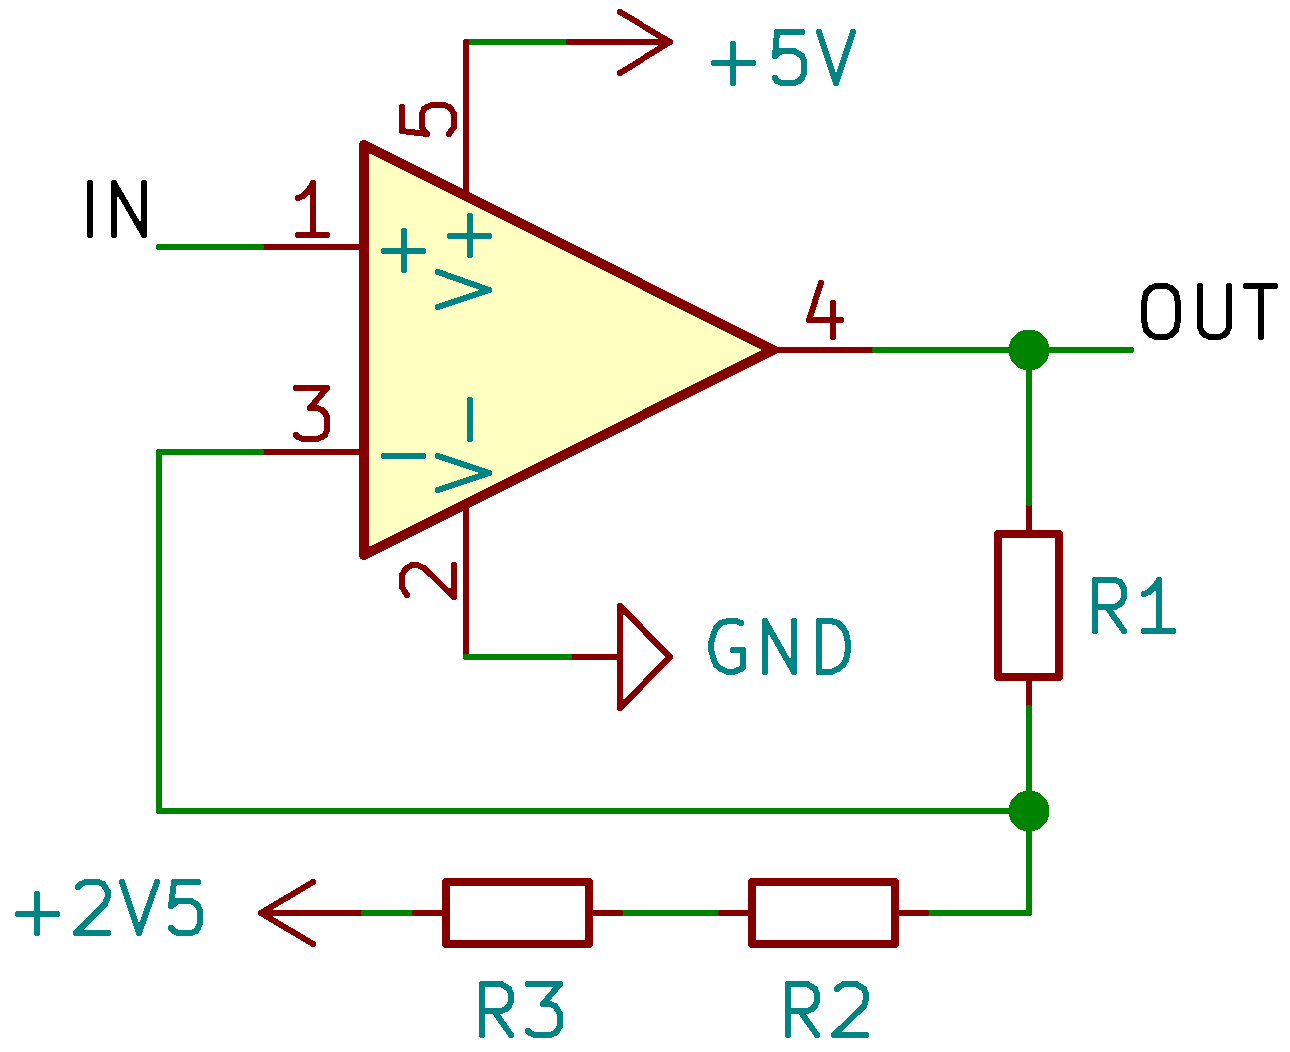
\includegraphics[width=\textwidth]{gain_circuit}
	\caption{The non-inverting amplifier circuit.}
	\label{fig:non-inverting-op-amp}
\end{subfigure}
\hfill
\begin{subfigure}[c]{0.45\textwidth}
	\centering
	\vfill
	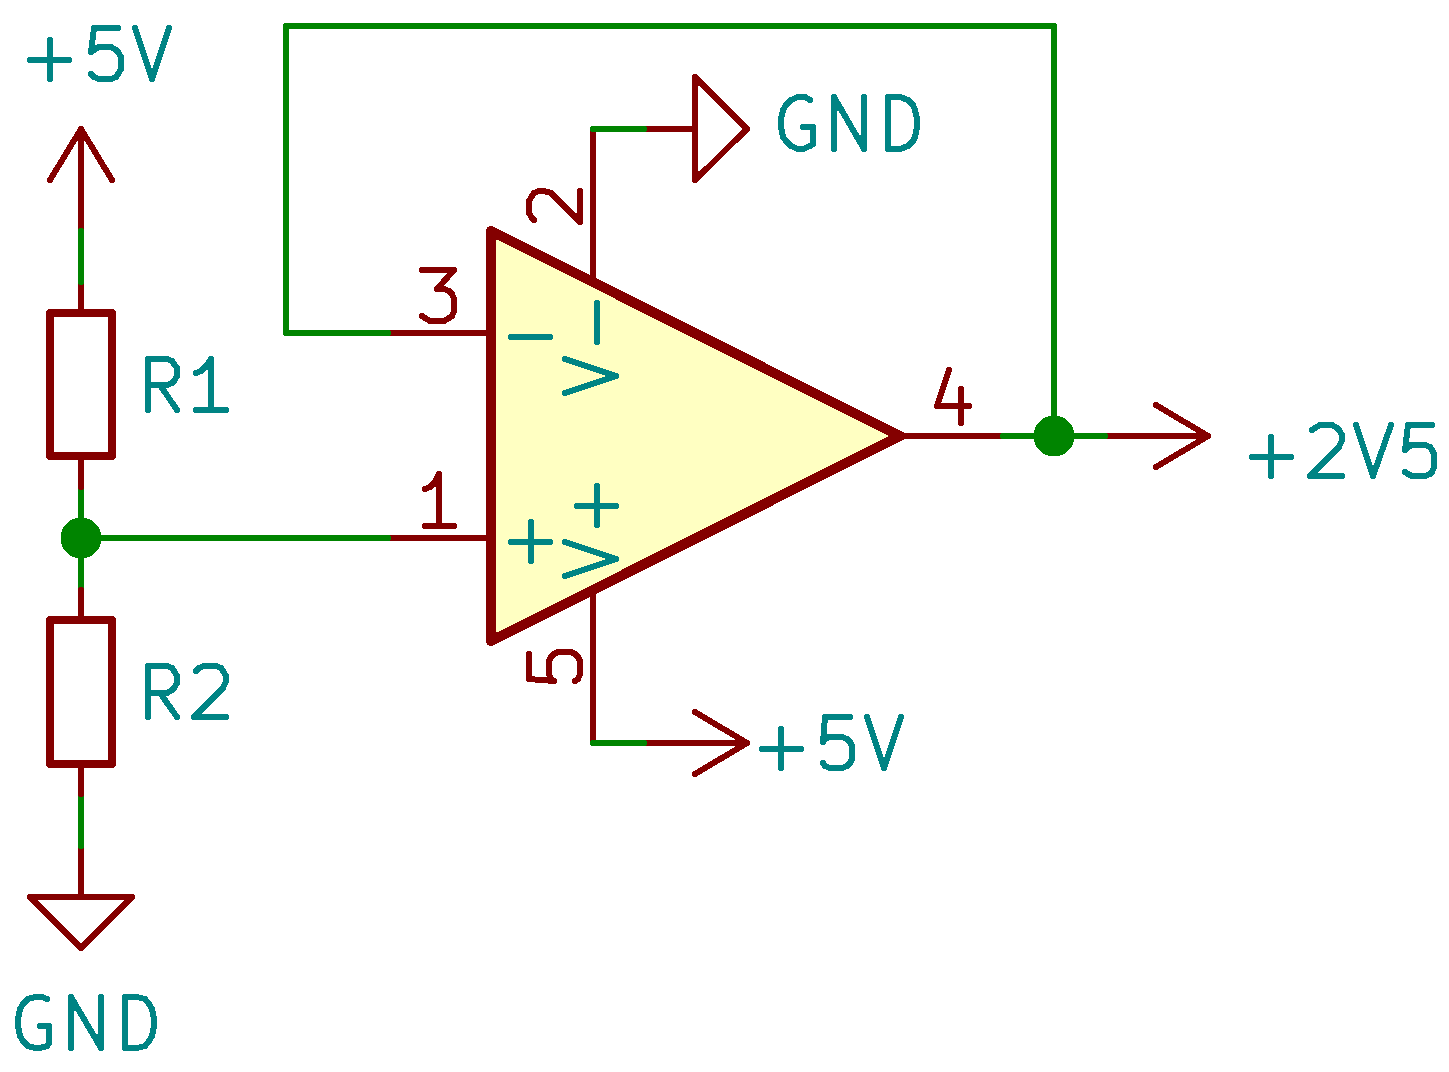
\includegraphics[width=\textwidth]{virtual_ground_circuit}
	\vfill
	\caption{The virtual ground circuit.}
	\label{fig:half-supply}
\end{subfigure}

\caption{The operational amplifer circuits used.}
\end{figure}

The op-amps are required to switch to a low power mode when no ADC readings are taking place.
Due to physical size constraints and part availability we have opted to drive the positive supply rail down to the level of the negative supply rail to achieve a low power state.
This is done with a CMOS inverter IC.
The main drawback of this method is the start-up time to enable the op-amps.
The sum of the time taken to switch the op-amp back on is $\SI{50}{\micro\second}$ (this is a phase angle of $\SI{7.2}{\degree}$ with respect to the AC signal).

The source impedance is specified as being less than $\SI{100}{\ohm}$.
A input impedance that is at least an order of magnitude higher than the source impedance is required for maximum voltage transfer and minimum current drain.
$Z_i = \SI{1}{\kilo\ohm}$ was decided upon, because it is 10 times higher than the worst-case source impedance.
Equations \ref{eq:r1} and \ref{eq:r2} show the derived formulae for the resistors based upon the given $Z_i$ and $A$ values.
\begin{align}
	R_1 &= Z_i A \label{eq:r1} \\
	R_2 + R_3 &= \frac{Z_i A}{A - 1} \label{eq:r2} \\[1em]
	\therefore R_1 = \SI{100}{\kilo\ohm}, R_2 &= \SI{1}{\kilo\ohm}, R_3 = \SI{10}{\ohm} \nonumber
\end{align}

12 of these non-inverting amplifier circuits are required for each daughterboard.
The LMV324 (\textcolor{red}{add citation}) selected as it has four op-amp circuits in one package, reducing the amount of space used on the board and the overall cost.
An additional op-amp package configured as a unity gain amplifer produces the half-rail reference from a voltage divider input.
High value resistors are required in the divider (typically $\SI{100}{\kilo\ohm}$ to prevent excessive static current drain.
However these produce greater thermal noise, especially at high ambient temperatures, which is undesirable for ADC applications.
Hence two $\SI{2.5}{\kilo\ohm}$ resistors balance the noise with a static current drain of $\SI{1}{\milli\ampere}$

Thermal calculations (\textcolor{red}{add reference to appendix}) show that the op-amps will supply minimal current into the microprocessor's ADC inputs.
Thus their power dissapation is relatively low.
The power dissapation is a function of the difference between supply voltage to output voltage, output voltage difference to ground (for single supply devices) and the output current.
With low power dissapation, there is a comfortable margin between the ambient temperature of $\SI{105}{\degreeCelsius}$, the junction operating temperature of $\SI{125}{\degreeCelsius}$, and the device absolute maximum of $\SI{150}{\degreeCelsius}$.
Additionally the worst case quiescent current is $\SI{150}{\micro\ampere}$.